\documentclass[10pt]{beamer}


\usepackage[utf8]{inputenc}
\usepackage[brazil]{babel}
\usepackage{graphicx}		% utilizado para inserir gráfico

\usepackage{verbatim}      % Para comentario em bloco

% Usado para incluir código
\usepackage{listings}
% Needed to use citations.
\usepackage{cite}

\usetheme{Copenhagen}
\usecolortheme{lccv}
\setbeamertemplate{background}{
\includegraphics[width=\paperwidth]{./figuras/background_lccv.jpg}}
%\setbeamercovered{transparent}

\title[]{eXtreme Programming}
\author[]{Baltazar Tavares Vanderlei\\
Dielson Sales de Carvalho\\
Priscylla Silva\\
Vinícius dos Santos Oliveira}
%\date{\today}
\institute[2013]{Instituto de Computação - IC/UFAL}

\begin{document}

\newcommand{\til}{\~{}}

\frame{\titlepage}
\begin{frame}[t]
  \frametitle{Sumário}
  \tableofcontents[framebreaks]
  % \tableofcontents[pausesections]
\end{frame}

% Perfumaria sobre o sumário ser mostrado a cada passagem de sessão e sub-sessão.
\AtBeginSection[]{
  \begin{frame}[t]
    \frametitle{Sumário}
    \tableofcontents[currentsection]
  \end{frame}
}

\AtBeginSubsection[]{
  \begin{frame}[t]
    \frametitle{Sumário}
    \tableofcontents[currentsubsection]
  \end{frame}
}


%%%%%%%%%%%%%%%%%%%%%%%%%%%%%%%%%%%%%%%%%%%%%%%%%%%%%%%%%%%%%%%%%
\section{XP (eXtreme Programming)}

\subsection{Visão Geral}

\begin{frame}
  \frametitle{Visão Geral quanto ao tempo}
  \begin{figure}
    \centering
%    \makebox[\textwidth]{\includegraphics[width=\paperwidth]{./figuras/visao_geral_tempo.png}}
    \makebox[\textheight]{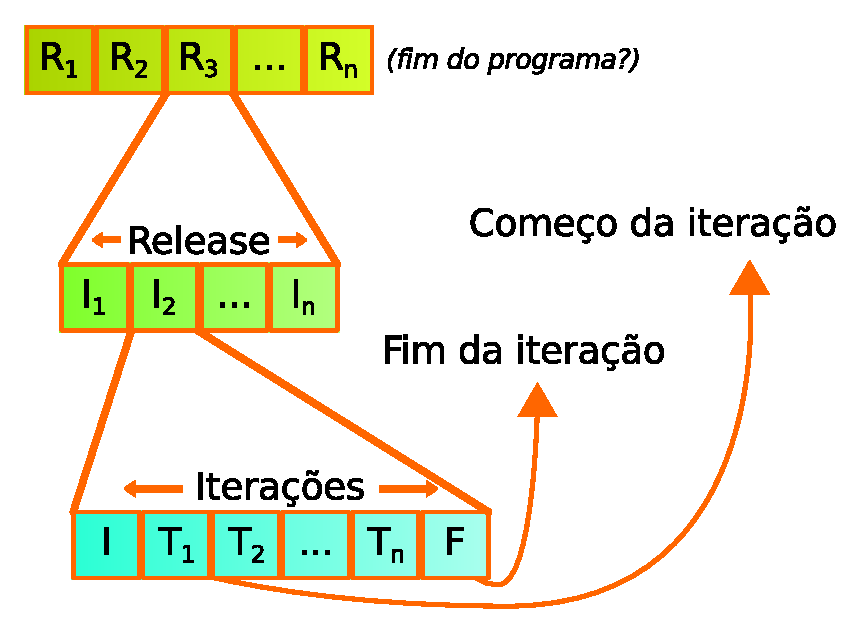
\includegraphics[scale=0.65]{./figuras/visao_geral_tempo.pdf}}
  \end{figure}
\end{frame}


\begin{frame}
  \frametitle{Visão geral}
  \begin{itemize}%[<+->]
  \item \textbf{Releases}
    \begin{block}{}
      \textbf{Levam meses}, são compostas de \textbf{iterações}
    \end{block}
  \item \textbf{Iterações}
    \begin{block}{}
      São periodos de poucas semanas(tipicamente, de \textbf{1 a 4 semanas}), são compostas de \textbf{tarefas}
    \end{block}
  \item \textbf{Tarefas}
    \begin{block}{}
      São \textbf{atividades basicas}, devem durar idealmente \textbf{1 dia de trabalho}, mas normalmente duram mais.
    \end{block}
  \end{itemize}
\end{frame}


\subsection{Releases}

\begin{frame}
%  \frametitle{Releases}
  \begin{figure}
    \centering
%    \makebox[\textwidth]{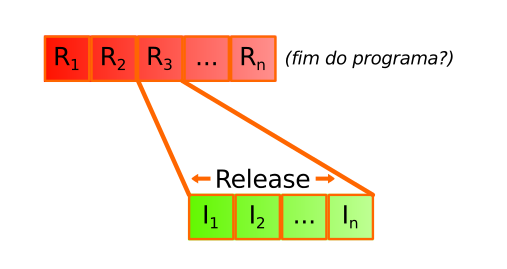
\includegraphics[width=\textwidth]{./figuras/ciclo_release.png}}
%    \makebox[\textwidth]{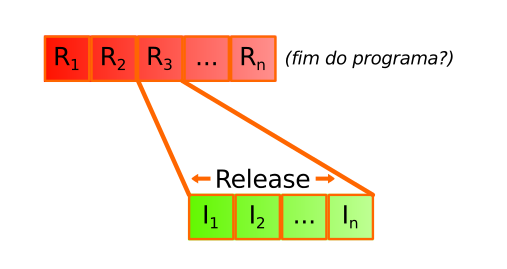
\includegraphics[scale=0.2]{./figuras/ciclo_release.png}}
    \makebox{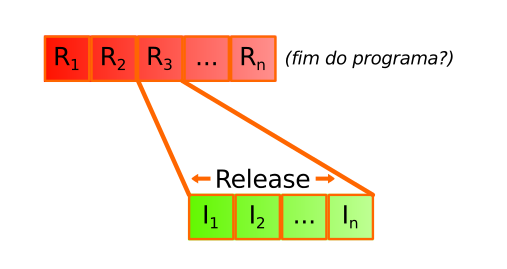
\includegraphics[scale=0.2]{./figuras/ciclo_release.png}}
  \end{figure}
  \begin{itemize}%[<+->]
    \item Refletir sobre o problemas, identificar e/ou propor soluções
    \item Cliente e equipe se reúnem para definir os temas
    \item Cliente controla o escopo, decidindo o que fazer ou adiar
    \item Normalmente, \textbf{3 meses}
  \end{itemize}
\end{frame}

\subsection{Iterações}

\begin{frame}
%  \frametitle{Iterações}
  \begin{itemize}%[<+->]
    \item Incremento projetado, programado, testado e entregue
    \item Ponto de avaliação, re-avaliação, feedback, interação com a satisfação do cliente e mudanças.
    \item Esse codigo vai ser aprimorado nas proximas iterações, mas é codigo funcional
    \item No inicio, Jogo do planejamento
    \item No final, o cliente tem a oportunidade de utilizar e avaliar o que foi produzido
    \item Normalmente, \textbf{1 semana}
  \end{itemize}
\end{frame}

\begin{frame}
%  \frametitle{Iterações}
  \begin{figure}
    \centering
    \makebox[\textwidth]{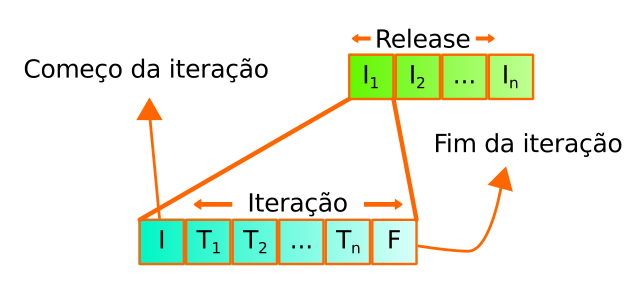
\includegraphics[width=\paperwidth]{./figuras/ciclo_iteracoes.png}}
  \end{figure}
\end{frame}

\begin{frame}
  \frametitle{Jogo do planejamento}
    \begin{block}{O cliente}
      \begin{itemize}%[<+->]
        \item Define as histórias(\textbf{User Story})
        \item Decide qual o valor de negócio de cada história
        \item Decide que histórias serão construídas no release
      \end{itemize}
    \end{block}
    \pause
    \begin{block}{Os programadores}
      \begin{itemize}%[<+->]
        \item Estimam quanto tempo será necessário para construir cada história, com base em experiencias passadas
        \item Advertem o cliente sobre riscos técnicos significativos
        \item Medem o progresso da equipe para fornecer um orçamento geral para o cliente
      \end{itemize}
    \end{block}
\end{frame}


\begin{frame}
  \frametitle{Final da Iteração}
  \begin{itemize}%[<+->]
    \item Testes de aceitação
    \item Entrega de software para o cliente
    \item Cliente tem oportunidade de testar e avaliar
  \end{itemize}
  \begin{block}{}
Com base nos resultados, reúne-se novamente com a equipe e estabelece novas prioridades de acordo com o que acabou de aprender com o software e com aquilo que já imaginava ser necessário produzir ao longo do restante do projeto.
  \end{block}
\end{frame}



\subsection{Tarefas}
\begin{frame}
  \begin{itemize}
  \item Compomente basico
  \item É a implementação de uma User story pelo par de programadores
  \item Testes!
  \item Executada de acordo com os valores e atividades do XP
  \end{itemize}
\end{frame}



\subsection{Valores}
\begin{frame}
  \frametitle{Valores}
  \begin{itemize}
  \item Comunicação
  \item Simplicidade
  \item Feedback
  \item Coragem
  \item Respeito
  \end{itemize}
\end{frame}

\subsection{Práticas do XP}
\begin{frame}
%  \frametitle{Práticas do XP}
  \begin{itemize}
  \item Cliente Presente
  \item Jogo do Planejamento
  \item Stand Up Meeting
  \item Programação em Pares
  \item Releases Curtos
  \item Desenvolvimento guiado por Testes
  \item Refactoring
  \item Código Coletivo
  \item Código Padronizado
  \item Integração Contínua
  \item Ritmo Sustentável
  \item Metáfora
  \end{itemize}
\end{frame}

\begin{frame}
  \frametitle{Cliente Presente}
  \begin{itemize}
  \item Parte da equipe
  \item Controla as tarefas de cada release baseadas no valor de negócio
  \item Feedback imediato
  \end{itemize}
\end{frame}

\begin{frame}
  \frametitle{Jogo do Planejamento}
  \begin{itemize}
  \item Mais importante primeiro
  \item Necessidades concretas
  \item Software funcionando em primeiro lugar
  \end{itemize}
\end{frame}

\begin{comment}

\begin{frame}
  \frametitle{Visão de alto nível}
  \begin{itemize}%[<+->]
  \item Boas práticas levadas ao extremo
    \begin{itemize}
    \item Envolvimento com o cliente
    \item TDD e revisão de código
    \item Entrega incremental
    \item Simplicidade
    \end{itemize}
  \end{itemize}
\end{frame}

\end{comment}

\begin{frame}
  \frametitle{Programação}
  \begin{itemize}
  \item Sem código, não há produto
  \item Pode ser usado para auxiliar a comunicação
  \end{itemize}
\end{frame}

\begin{frame}
  \frametitle{Testes}
  \begin{itemize}
  \item Testes unitários
  \item Testes de aceitação
  \item Testes de integração
  \end{itemize}
\end{frame}

\begin{frame}
  \frametitle{Escutar}
  Programadores devem escutar o que os clientes precisam que o sistema faça.

  \pause
  Programadores devem entender o sistema bem o suficiente para dar feedback
  sobre os detalhes técnicos de como o problema pode ser resolvido.
\end{frame}

\begin{frame}
  \frametitle{Projeto}
  \begin{itemize}
  \item Sistema muito complexo
  \item As dependências não ficam claras
  \end{itemize}
\end{frame}
%%%%%%%%%%%%%%%%%%%%%%%%%%%%%%%%%%%%%%%%%%%%%%%%%

\section{Quando não usar XP}


\begin{frame}
  \frametitle{Itens polêmicos}
  \begin{itemize}
  \item Requerimentos instáveis
  \item Documentação menos completa, quando comparada a processos pesados
  \item Programar para o agora pode tornar o trabalho de amanhã mais pesado
  \item Sistemas críticos
  \end{itemize}
\end{frame}


\begin{frame}
  \frametitle{Quando não usar XP}
  \begin{itemize}
  \item Equipe com cultura tradicional de desenvolvimento de software
  \item Equipes Grandes ($>$12)
  \item Tecnologias usadas não permitem TDD
  \item Espaço Físico invabiliza a utilização
  \item Clientes exigem documentação rigorosa
  \item Clientes não possuem tempo disponível
  \end{itemize}
\end{frame}

%%%%%%%%%%%%%%%%%%%%%%%%%%%%%%%%%%%%%%%%%%%%%%%%%
\section{Casos de uso}
\begin{frame}
  \frametitle{Companhias que Utilizam o XP}
  \textbf{Brasileiras:}
  \begin{itemize}
    \item Improve It (RJ)
    \item Globo (RJ)
    \item BrasilTelecom (DF)
    \item Embrapa Informática (SP)
  \end{itemize}
  \textbf{Internacionais:}
  \begin{itemize}
    \item Blizzard
    \item Sabre Airline Solutions
    \item Arshin
    \item Motorola, inc.
  \end{itemize}
\end{frame}




\begin{comment}

Kent Beck em 1997, surgiu o XP.

2001, fevereiro, utah:

       Surgiu o manifesto agil

manifesto agil:

O manifesto estabelece um conjunto de valores que são adotados nos projetos ágeis:

¿ Indivíduos e interações ao invés de processos e ferramentas;

¿ Software funcionando ao invés de documentação abrangente;

¿ Colaboração com o cliente ao invés de negociação de contratos;

¿ Responder a mudanças ao invés de seguir um plano.



XP:



Conjunto reduzido de práticas de desenvolvimento que se organizam em torno de quatro valores básicos.


O que são os valores?

%http://improveit.com.br/xp/valores

    Comunicação

    Coragem

    Feedback

    Respeito

    Simplicidade


O que são praticas?

%http://improveit.com.br/xp/praticas


XP quanto ao tempo:

Releases: as releases tomam meses, são compostas de iterações

Iterações: São periodos de poucas semanas(tipicamente, de 1 a 4 semanas), são compostas de tarefas

Tarefas: São atividades basicas, devem durar idealmente 1 dia de trabalho, mas de vez em quando duram um pouco mais.


Em cada release:

O cliente controla o escopo, decidindo o que fazer e o que adiar, de modo a prover o melhor release possível na data acertada. O trabalho se encaixa no cronograma baseado no valor para o negócio, dificuldade e a velocidade de implementação da equipe.

representa um marco no tempo no qual um conjunto coeso de funcionalidades é finalizado e lançado para consumo de seus usuários.


Em cada iteração:

um incremento de software útil que é projetado, programado, testado, integrado e entregue durante um espaço de tempo curto e fixo. á aprimorado em iterações futuras, mas se trata de código funcional.

É um ponto de avaliação, re-avaliação, feedback, interação com a satisfação do cliente e mudanças.

1) Jogo do  planejamento

O cliente:
* Define as histórias;
* Decide qual o valor de negócio de cada história
* Decide que histórias serão construídas no release.

Os programadores:
* Estimam quanto tempo será necessário para construir cada história;
* Advertem o cliente sobre riscos técnicos significativos
* Medem o progresso da equipe para fornecer um orçamento geral para o cliente (BECK & FOWLER, 2001, p.40, tradução nossa).

O produto são User story

%http://www.slideshare.net/MCPTECNOLOGIA/user-stories-5564287

2) Atividades diarias

** Vamos chegar lá .....

3)


%http://www.slideshare.net/dwildt/conhecendo-o-extreme-programming


%http://www.naphta.com.br/xpmanager/xpmanager_projetoxp.jpg
\end{comment}


\end{document}
